% Options for packages loaded elsewhere
\PassOptionsToPackage{unicode}{hyperref}
\PassOptionsToPackage{hyphens}{url}
%
\documentclass[
]{book}
\usepackage{amsmath,amssymb}
\usepackage{lmodern}
\usepackage{ifxetex,ifluatex}
\ifnum 0\ifxetex 1\fi\ifluatex 1\fi=0 % if pdftex
  \usepackage[T1]{fontenc}
  \usepackage[utf8]{inputenc}
  \usepackage{textcomp} % provide euro and other symbols
\else % if luatex or xetex
  \usepackage{unicode-math}
  \defaultfontfeatures{Scale=MatchLowercase}
  \defaultfontfeatures[\rmfamily]{Ligatures=TeX,Scale=1}
\fi
% Use upquote if available, for straight quotes in verbatim environments
\IfFileExists{upquote.sty}{\usepackage{upquote}}{}
\IfFileExists{microtype.sty}{% use microtype if available
  \usepackage[]{microtype}
  \UseMicrotypeSet[protrusion]{basicmath} % disable protrusion for tt fonts
}{}
\makeatletter
\@ifundefined{KOMAClassName}{% if non-KOMA class
  \IfFileExists{parskip.sty}{%
    \usepackage{parskip}
  }{% else
    \setlength{\parindent}{0pt}
    \setlength{\parskip}{6pt plus 2pt minus 1pt}}
}{% if KOMA class
  \KOMAoptions{parskip=half}}
\makeatother
\usepackage{xcolor}
\IfFileExists{xurl.sty}{\usepackage{xurl}}{} % add URL line breaks if available
\IfFileExists{bookmark.sty}{\usepackage{bookmark}}{\usepackage{hyperref}}
\hypersetup{
  pdftitle={CART microbiome analysis},
  pdfauthor={Anqi Dai},
  hidelinks,
  pdfcreator={LaTeX via pandoc}}
\urlstyle{same} % disable monospaced font for URLs
\usepackage{color}
\usepackage{fancyvrb}
\newcommand{\VerbBar}{|}
\newcommand{\VERB}{\Verb[commandchars=\\\{\}]}
\DefineVerbatimEnvironment{Highlighting}{Verbatim}{commandchars=\\\{\}}
% Add ',fontsize=\small' for more characters per line
\usepackage{framed}
\definecolor{shadecolor}{RGB}{248,248,248}
\newenvironment{Shaded}{\begin{snugshade}}{\end{snugshade}}
\newcommand{\AlertTok}[1]{\textcolor[rgb]{0.94,0.16,0.16}{#1}}
\newcommand{\AnnotationTok}[1]{\textcolor[rgb]{0.56,0.35,0.01}{\textbf{\textit{#1}}}}
\newcommand{\AttributeTok}[1]{\textcolor[rgb]{0.77,0.63,0.00}{#1}}
\newcommand{\BaseNTok}[1]{\textcolor[rgb]{0.00,0.00,0.81}{#1}}
\newcommand{\BuiltInTok}[1]{#1}
\newcommand{\CharTok}[1]{\textcolor[rgb]{0.31,0.60,0.02}{#1}}
\newcommand{\CommentTok}[1]{\textcolor[rgb]{0.56,0.35,0.01}{\textit{#1}}}
\newcommand{\CommentVarTok}[1]{\textcolor[rgb]{0.56,0.35,0.01}{\textbf{\textit{#1}}}}
\newcommand{\ConstantTok}[1]{\textcolor[rgb]{0.00,0.00,0.00}{#1}}
\newcommand{\ControlFlowTok}[1]{\textcolor[rgb]{0.13,0.29,0.53}{\textbf{#1}}}
\newcommand{\DataTypeTok}[1]{\textcolor[rgb]{0.13,0.29,0.53}{#1}}
\newcommand{\DecValTok}[1]{\textcolor[rgb]{0.00,0.00,0.81}{#1}}
\newcommand{\DocumentationTok}[1]{\textcolor[rgb]{0.56,0.35,0.01}{\textbf{\textit{#1}}}}
\newcommand{\ErrorTok}[1]{\textcolor[rgb]{0.64,0.00,0.00}{\textbf{#1}}}
\newcommand{\ExtensionTok}[1]{#1}
\newcommand{\FloatTok}[1]{\textcolor[rgb]{0.00,0.00,0.81}{#1}}
\newcommand{\FunctionTok}[1]{\textcolor[rgb]{0.00,0.00,0.00}{#1}}
\newcommand{\ImportTok}[1]{#1}
\newcommand{\InformationTok}[1]{\textcolor[rgb]{0.56,0.35,0.01}{\textbf{\textit{#1}}}}
\newcommand{\KeywordTok}[1]{\textcolor[rgb]{0.13,0.29,0.53}{\textbf{#1}}}
\newcommand{\NormalTok}[1]{#1}
\newcommand{\OperatorTok}[1]{\textcolor[rgb]{0.81,0.36,0.00}{\textbf{#1}}}
\newcommand{\OtherTok}[1]{\textcolor[rgb]{0.56,0.35,0.01}{#1}}
\newcommand{\PreprocessorTok}[1]{\textcolor[rgb]{0.56,0.35,0.01}{\textit{#1}}}
\newcommand{\RegionMarkerTok}[1]{#1}
\newcommand{\SpecialCharTok}[1]{\textcolor[rgb]{0.00,0.00,0.00}{#1}}
\newcommand{\SpecialStringTok}[1]{\textcolor[rgb]{0.31,0.60,0.02}{#1}}
\newcommand{\StringTok}[1]{\textcolor[rgb]{0.31,0.60,0.02}{#1}}
\newcommand{\VariableTok}[1]{\textcolor[rgb]{0.00,0.00,0.00}{#1}}
\newcommand{\VerbatimStringTok}[1]{\textcolor[rgb]{0.31,0.60,0.02}{#1}}
\newcommand{\WarningTok}[1]{\textcolor[rgb]{0.56,0.35,0.01}{\textbf{\textit{#1}}}}
\usepackage{longtable,booktabs,array}
\usepackage{calc} % for calculating minipage widths
% Correct order of tables after \paragraph or \subparagraph
\usepackage{etoolbox}
\makeatletter
\patchcmd\longtable{\par}{\if@noskipsec\mbox{}\fi\par}{}{}
\makeatother
% Allow footnotes in longtable head/foot
\IfFileExists{footnotehyper.sty}{\usepackage{footnotehyper}}{\usepackage{footnote}}
\makesavenoteenv{longtable}
\usepackage{graphicx}
\makeatletter
\def\maxwidth{\ifdim\Gin@nat@width>\linewidth\linewidth\else\Gin@nat@width\fi}
\def\maxheight{\ifdim\Gin@nat@height>\textheight\textheight\else\Gin@nat@height\fi}
\makeatother
% Scale images if necessary, so that they will not overflow the page
% margins by default, and it is still possible to overwrite the defaults
% using explicit options in \includegraphics[width, height, ...]{}
\setkeys{Gin}{width=\maxwidth,height=\maxheight,keepaspectratio}
% Set default figure placement to htbp
\makeatletter
\def\fps@figure{htbp}
\makeatother
\setlength{\emergencystretch}{3em} % prevent overfull lines
\providecommand{\tightlist}{%
  \setlength{\itemsep}{0pt}\setlength{\parskip}{0pt}}
\setcounter{secnumdepth}{5}
\usepackage{booktabs}
\ifluatex
  \usepackage{selnolig}  % disable illegal ligatures
\fi
\usepackage[]{natbib}
\bibliographystyle{apalike}

\title{CART microbiome analysis}
\author{Anqi Dai}
\date{2021-07-14}

\begin{document}
\maketitle

{
\setcounter{tocdepth}{1}
\tableofcontents
}
\hypertarget{prerequisites}{%
\chapter{Prerequisites}\label{prerequisites}}

\begin{Shaded}
\begin{Highlighting}[]
\FunctionTok{install.packages}\NormalTok{(}\StringTok{"bookdown"}\NormalTok{)}
\end{Highlighting}
\end{Shaded}

\hypertarget{intro}{%
\chapter{Introduction}\label{intro}}

You can label chapter and section titles using \texttt{\{\#label\}} after them, e.g., we can reference Chapter \ref{intro}. If you do not manually label them, there will be automatic labels anyway, e.g., Chapter \ref{methods}.

Figures and tables with captions will be placed in \texttt{figure} and \texttt{table} environments, respectively.

\begin{Shaded}
\begin{Highlighting}[]
\FunctionTok{par}\NormalTok{(}\AttributeTok{mar =} \FunctionTok{c}\NormalTok{(}\DecValTok{4}\NormalTok{, }\DecValTok{4}\NormalTok{, .}\DecValTok{1}\NormalTok{, .}\DecValTok{1}\NormalTok{))}
\FunctionTok{plot}\NormalTok{(pressure, }\AttributeTok{type =} \StringTok{\textquotesingle{}b\textquotesingle{}}\NormalTok{, }\AttributeTok{pch =} \DecValTok{19}\NormalTok{)}
\end{Highlighting}
\end{Shaded}

\begin{figure}

{\centering 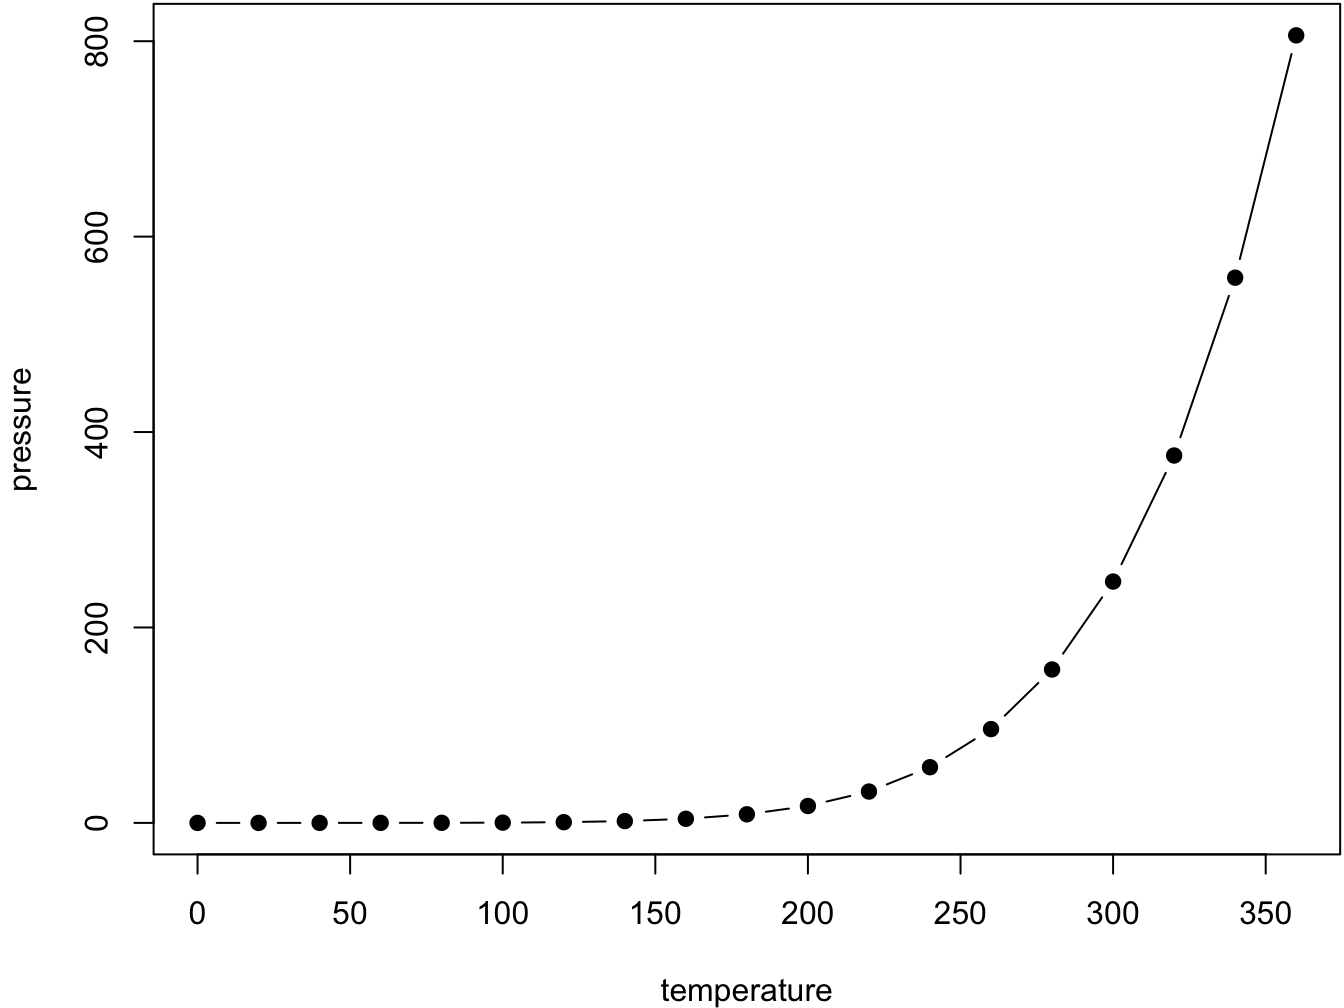
\includegraphics[width=0.8\linewidth]{analysis_files/figure-latex/nice-fig-1} 

}

\caption{Here is a nice figure!}\label{fig:nice-fig}
\end{figure}

Reference a figure by its code chunk label with the \texttt{fig:} prefix, e.g., see Figure \ref{fig:nice-fig}. Similarly, you can reference tables generated from \texttt{knitr::kable()}, e.g., see Table \ref{tab:nice-tab}.

\begin{Shaded}
\begin{Highlighting}[]
\NormalTok{knitr}\SpecialCharTok{::}\FunctionTok{kable}\NormalTok{(}
  \FunctionTok{head}\NormalTok{(iris, }\DecValTok{20}\NormalTok{), }\AttributeTok{caption =} \StringTok{\textquotesingle{}Here is a nice table!\textquotesingle{}}\NormalTok{,}
  \AttributeTok{booktabs =} \ConstantTok{TRUE}
\NormalTok{)}
\end{Highlighting}
\end{Shaded}

\begin{table}

\caption{\label{tab:nice-tab}Here is a nice table!}
\centering
\begin{tabular}[t]{rrrrl}
\toprule
Sepal.Length & Sepal.Width & Petal.Length & Petal.Width & Species\\
\midrule
5.1 & 3.5 & 1.4 & 0.2 & setosa\\
4.9 & 3.0 & 1.4 & 0.2 & setosa\\
4.7 & 3.2 & 1.3 & 0.2 & setosa\\
4.6 & 3.1 & 1.5 & 0.2 & setosa\\
5.0 & 3.6 & 1.4 & 0.2 & setosa\\
\addlinespace
5.4 & 3.9 & 1.7 & 0.4 & setosa\\
4.6 & 3.4 & 1.4 & 0.3 & setosa\\
5.0 & 3.4 & 1.5 & 0.2 & setosa\\
4.4 & 2.9 & 1.4 & 0.2 & setosa\\
4.9 & 3.1 & 1.5 & 0.1 & setosa\\
\addlinespace
5.4 & 3.7 & 1.5 & 0.2 & setosa\\
4.8 & 3.4 & 1.6 & 0.2 & setosa\\
4.8 & 3.0 & 1.4 & 0.1 & setosa\\
4.3 & 3.0 & 1.1 & 0.1 & setosa\\
5.8 & 4.0 & 1.2 & 0.2 & setosa\\
\addlinespace
5.7 & 4.4 & 1.5 & 0.4 & setosa\\
5.4 & 3.9 & 1.3 & 0.4 & setosa\\
5.1 & 3.5 & 1.4 & 0.3 & setosa\\
5.7 & 3.8 & 1.7 & 0.3 & setosa\\
5.1 & 3.8 & 1.5 & 0.3 & setosa\\
\bottomrule
\end{tabular}
\end{table}

You can write citations, too. For example, we are using the \textbf{bookdown} package \citep{R-bookdown} in this sample book, which was built on top of R Markdown and \textbf{knitr} \citep{xie2015}.

\hypertarget{fig-2}{%
\chapter{Fig 2}\label{fig-2}}

\hypertarget{b-stacked-bar-chart.}{%
\section{2B: stacked bar chart.}\label{b-stacked-bar-chart.}}

\begin{Shaded}
\begin{Highlighting}[]
\FunctionTok{library}\NormalTok{(tidyverse)}
\FunctionTok{library}\NormalTok{(vdbR)}
\FunctionTok{library}\NormalTok{(ggpubr)}
\FunctionTok{connect\_database}\NormalTok{(}\StringTok{\textquotesingle{}\textasciitilde{}/dbConfig.txt\textquotesingle{}}\NormalTok{)}
\FunctionTok{get\_table\_from\_database}\NormalTok{(}\StringTok{"asv\_annotation\_blast\_color\_ag"}\NormalTok{);}
\end{Highlighting}
\end{Shaded}

\begin{Shaded}
\begin{Highlighting}[]
\CommentTok{\# my table of the CART stool cohort}
\NormalTok{stb }\OtherTok{\textless{}{-}} \FunctionTok{read\_csv}\NormalTok{(}\StringTok{\textquotesingle{}data/amplicon/stool/combined\_2\_meta.csv\textquotesingle{}}\NormalTok{)}
\CommentTok{\# get the counts from database and also the color for the asv }
\NormalTok{counts\_data }\OtherTok{\textless{}{-}} \FunctionTok{get\_counts\_subset}\NormalTok{(stb}\SpecialCharTok{$}\NormalTok{sampleid)}
\end{Highlighting}
\end{Shaded}

\begin{Shaded}
\begin{Highlighting}[]
\NormalTok{dat }\OtherTok{\textless{}{-}}\NormalTok{ counts\_data }\SpecialCharTok{\%\textgreater{}\%} 
  \FunctionTok{select}\NormalTok{(asv\_key}\SpecialCharTok{:}\NormalTok{count\_total, count\_relative) }\SpecialCharTok{\%\textgreater{}\%} 
  \FunctionTok{left\_join}\NormalTok{(asv\_annotation\_blast\_color\_ag }\SpecialCharTok{\%\textgreater{}\%} 
              \FunctionTok{select}\NormalTok{(asv\_key,color\_label\_group\_distinct), }\AttributeTok{by =} \StringTok{"asv\_key"}\NormalTok{)}
\CommentTok{\# there are some ASVs that don\textquotesingle{}t have a color with it, but can use the color for the genus level}
\NormalTok{color\_group }\OtherTok{\textless{}{-}}\NormalTok{ dat }\SpecialCharTok{\%\textgreater{}\%} 
  \FunctionTok{split}\NormalTok{(}\FunctionTok{is.na}\NormalTok{(.}\SpecialCharTok{$}\NormalTok{color\_label\_group\_distinct))}
\CommentTok{\# find the genus for these asv}
\FunctionTok{get\_table\_from\_database}\NormalTok{(}\StringTok{\textquotesingle{}asv\_annotation\_blast\_ag\textquotesingle{}}\NormalTok{)}
\NormalTok{no\_color }\OtherTok{\textless{}{-}}\NormalTok{ color\_group }\SpecialCharTok{\%\textgreater{}\%} 
  \FunctionTok{pluck}\NormalTok{(}\StringTok{\textquotesingle{}TRUE\textquotesingle{}}\NormalTok{) }\SpecialCharTok{\%\textgreater{}\%} 
  \FunctionTok{distinct}\NormalTok{(asv\_key) }\SpecialCharTok{\%\textgreater{}\%} 
  \FunctionTok{inner\_join}\NormalTok{(asv\_annotation\_blast\_ag }\SpecialCharTok{\%\textgreater{}\%} 
               \FunctionTok{select}\NormalTok{(asv\_key, genus)) }
\CommentTok{\# find the colors for these genera}
\NormalTok{genera\_colors }\OtherTok{\textless{}{-}}\NormalTok{ no\_color }\SpecialCharTok{\%\textgreater{}\%} 
  \FunctionTok{distinct}\NormalTok{(genus) }\SpecialCharTok{\%\textgreater{}\%} 
  \FunctionTok{inner\_join}\NormalTok{(asv\_annotation\_blast\_color\_ag }\SpecialCharTok{\%\textgreater{}\%} 
               \FunctionTok{distinct}\NormalTok{(genus, color\_label\_group\_distinct))}
\CommentTok{\# the full df for the no color genera}
\NormalTok{no\_color\_df }\OtherTok{\textless{}{-}}\NormalTok{ no\_color }\SpecialCharTok{\%\textgreater{}\%} 
  \FunctionTok{left\_join}\NormalTok{(genera\_colors)}
\NormalTok{no\_color\_df\_full }\OtherTok{\textless{}{-}}\NormalTok{ color\_group }\SpecialCharTok{\%\textgreater{}\%} 
  \FunctionTok{pluck}\NormalTok{(}\StringTok{\textquotesingle{}TRUE\textquotesingle{}}\NormalTok{) }\SpecialCharTok{\%\textgreater{}\%} 
  \FunctionTok{select}\NormalTok{(}\SpecialCharTok{{-}}\NormalTok{color\_label\_group\_distinct) }\SpecialCharTok{\%\textgreater{}\%} 
  \FunctionTok{left\_join}\NormalTok{(no\_color\_df }\SpecialCharTok{\%\textgreater{}\%} 
              \FunctionTok{select}\NormalTok{(}\SpecialCharTok{{-}}\NormalTok{ genus))}
  
\CommentTok{\# so if the genus is unknown then it\textquotesingle{}s gonna be assigned "other" gray color  }
\CommentTok{\# the question is do we go one taxa level higher or make a new color base and shades for the new asv}
\CommentTok{\# after discussing with Tsoni, we decided that it\textquotesingle{}s ok to assign gray to the unknown genus }
\CommentTok{\# merge the new no\_color\_df\_full to the original df}
\NormalTok{dat }\OtherTok{\textless{}{-}} \FunctionTok{bind\_rows}\NormalTok{(}
\NormalTok{  no\_color\_df\_full,}
\NormalTok{  color\_group }\SpecialCharTok{\%\textgreater{}\%} 
    \FunctionTok{pluck}\NormalTok{(}\StringTok{\textquotesingle{}FALSE\textquotesingle{}}\NormalTok{)}
\NormalTok{)   }
\NormalTok{dat }\SpecialCharTok{\%\textgreater{}\%}  \FunctionTok{write\_csv}\NormalTok{(}\StringTok{\textquotesingle{}data/the\_data\_to\_make\_panel\_B.csv\textquotesingle{}}\NormalTok{)}
\end{Highlighting}
\end{Shaded}

\begin{Shaded}
\begin{Highlighting}[]
\CommentTok{\# the color palette (inherited from Ying, used in lots of project in our lab, the palette used in the NEJM paper Fig 2D https://www.nejm.org/doi/full/10.1056/NEJMoa1900623)}
\NormalTok{asv\_color\_set }\OtherTok{\textless{}{-}}\NormalTok{ asv\_annotation\_blast\_color\_ag }\SpecialCharTok{\%\textgreater{}\%} 
  \FunctionTok{distinct}\NormalTok{(color,color\_label\_group\_distinct,color\_label\_group,color\_base) }\SpecialCharTok{\%\textgreater{}\%} 
  \FunctionTok{select}\NormalTok{(color\_label\_group\_distinct, color) }\SpecialCharTok{\%\textgreater{}\%} 
  \FunctionTok{deframe}\NormalTok{()}
\end{Highlighting}
\end{Shaded}

\begin{Shaded}
\begin{Highlighting}[]
\CommentTok{\# calculate the beta diversity between the samples which deicide the order of the samples in the plot}
\NormalTok{cbd }\OtherTok{\textless{}{-}} \FunctionTok{compute\_beta\_diversity\_and\_tsne}\NormalTok{(}\AttributeTok{sampleid =}\NormalTok{ dat}\SpecialCharTok{$}\NormalTok{sampleid, }
                                      \AttributeTok{taxonomy =}\NormalTok{ dat}\SpecialCharTok{$}\NormalTok{color\_label\_group\_distinct,}
                                      \AttributeTok{count =}\NormalTok{ dat}\SpecialCharTok{$}\NormalTok{count);}
\CommentTok{\#compute beta diversity}
\NormalTok{cbd}\SpecialCharTok{$}\FunctionTok{compute\_beta\_diversity}\NormalTok{()}
\end{Highlighting}
\end{Shaded}

\begin{verbatim}
## Time:Composition_matrix:
## Time difference of 0.01128983 secs
## Time:Bray-Curtis matrix:
## Time difference of 0.002399921 secs
\end{verbatim}

\begin{Shaded}
\begin{Highlighting}[]
\CommentTok{\#get beta diversity}
\NormalTok{d\_beta }\OtherTok{\textless{}{-}}\NormalTok{ cbd}\SpecialCharTok{$}\FunctionTok{get\_betadiversity}\NormalTok{() }
\CommentTok{\#compute hierarchical cluster}
\NormalTok{hc }\OtherTok{\textless{}{-}} \FunctionTok{hclust}\NormalTok{(}\FunctionTok{as.dist}\NormalTok{(d\_beta), }\AttributeTok{method =} \StringTok{\textquotesingle{}complete\textquotesingle{}}\NormalTok{)}
\NormalTok{dend }\OtherTok{\textless{}{-}} \FunctionTok{as.dendrogram}\NormalTok{(hc)}
\NormalTok{sample\_dendogram\_order }\OtherTok{\textless{}{-}} \FunctionTok{labels}\NormalTok{(dend)}


\CommentTok{\#  dividing the samples to lower and higher diversity }

\NormalTok{div\_order }\OtherTok{\textless{}{-}}\NormalTok{ stb }\SpecialCharTok{\%\textgreater{}\%} 
  \FunctionTok{arrange}\NormalTok{(simpson\_reciprocal) }\SpecialCharTok{\%\textgreater{}\%} 
  \FunctionTok{pull}\NormalTok{(sampleid)}
\DocumentationTok{\#\#\#}
\CommentTok{\# how about splitting the above dendrogram order into the low and higher diversity groups}
\NormalTok{div\_med }\OtherTok{\textless{}{-}} \FunctionTok{median}\NormalTok{(stb}\SpecialCharTok{$}\NormalTok{simpson\_reciprocal)}
\NormalTok{lower\_samp }\OtherTok{\textless{}{-}}\NormalTok{ stb }\SpecialCharTok{\%\textgreater{}\%} 
  \FunctionTok{filter}\NormalTok{(simpson\_reciprocal }\SpecialCharTok{\textless{}=}\NormalTok{ div\_med) }\SpecialCharTok{\%\textgreater{}\%} 
  \FunctionTok{pull}\NormalTok{(sampleid)}
\NormalTok{lower\_samp\_o }\OtherTok{\textless{}{-}}\NormalTok{ sample\_dendogram\_order[sample\_dendogram\_order }\SpecialCharTok{\%in\%}\NormalTok{ lower\_samp]}
\NormalTok{higher\_samp\_o }\OtherTok{\textless{}{-}}\NormalTok{ sample\_dendogram\_order[}\SpecialCharTok{!}\NormalTok{sample\_dendogram\_order }\SpecialCharTok{\%in\%}\NormalTok{ lower\_samp]}
\NormalTok{dat}\SpecialCharTok{$}\NormalTok{sampleid }\OtherTok{=} \FunctionTok{factor}\NormalTok{(dat}\SpecialCharTok{$}\NormalTok{sampleid,}\AttributeTok{levels =} \FunctionTok{c}\NormalTok{(lower\_samp\_o, higher\_samp\_o))}
\FunctionTok{ggplot}\NormalTok{(dat,}\FunctionTok{aes}\NormalTok{(sampleid, count\_relative, }\AttributeTok{fill =}\NormalTok{ color\_label\_group\_distinct) ) }\SpecialCharTok{+}
  \FunctionTok{geom\_bar}\NormalTok{(}\AttributeTok{stat =} \StringTok{"identity"}\NormalTok{, }\AttributeTok{position=}\StringTok{"fill"}\NormalTok{, }\AttributeTok{width =} \DecValTok{1}\NormalTok{) }\SpecialCharTok{+}
  \FunctionTok{theme\_classic}\NormalTok{() }\SpecialCharTok{+}
  \FunctionTok{labs}\NormalTok{(}\AttributeTok{title =} \StringTok{\textquotesingle{}\textquotesingle{}}\NormalTok{,}
       \AttributeTok{ylab =} \StringTok{\textquotesingle{}Relative counts\textquotesingle{}}\NormalTok{) }\SpecialCharTok{+}
  \FunctionTok{theme}\NormalTok{(}\AttributeTok{axis.text.x =} \FunctionTok{element\_text}\NormalTok{(}\AttributeTok{angle =} \DecValTok{90}\NormalTok{),}
        \AttributeTok{axis.text.y =} \FunctionTok{element\_blank}\NormalTok{(),}
        \AttributeTok{legend.position =} \StringTok{"none"}\NormalTok{) }\SpecialCharTok{+}
  \FunctionTok{scale\_fill\_manual}\NormalTok{(}\AttributeTok{values =}\NormalTok{ asv\_color\_set) }\SpecialCharTok{+}
  \FunctionTok{ggsave}\NormalTok{(}\StringTok{\textquotesingle{}figs/amplicon/stacked\_bar\_sorted\_with\_hclust\_lower\_and\_higher\_diversity.pdf\textquotesingle{}}\NormalTok{, }\AttributeTok{width =} \DecValTok{7}\NormalTok{, }\AttributeTok{height =} \DecValTok{5}\NormalTok{)}
\end{Highlighting}
\end{Shaded}

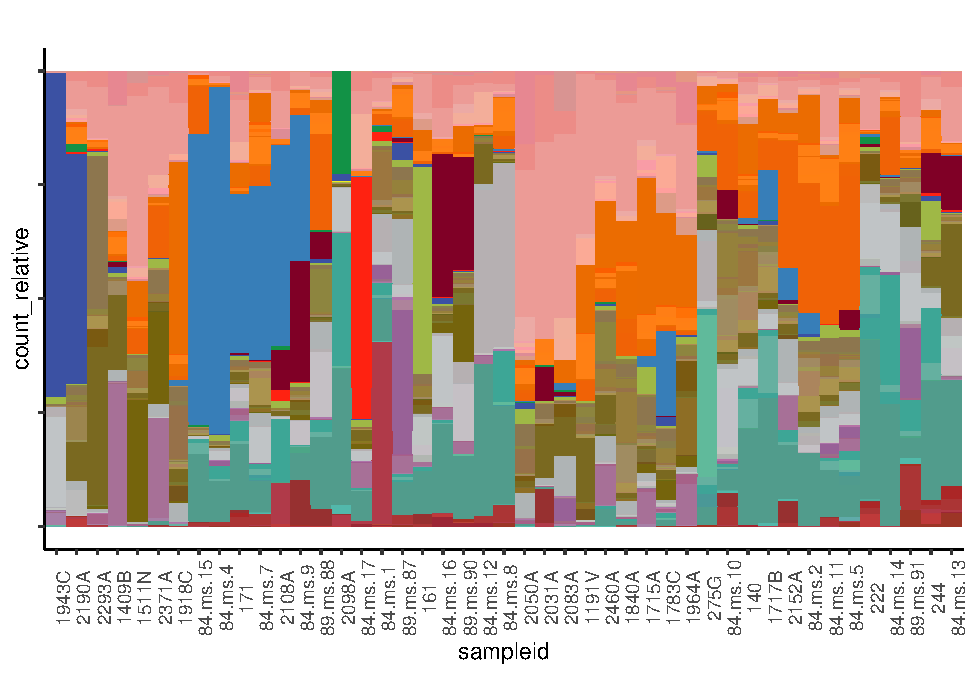
\includegraphics{analysis_files/figure-latex/unnamed-chunk-8-1.pdf}

\hypertarget{c-alpha-and-beta-diversity-between-cart-patients-and-healthy-volunteers}{%
\section{2C: alpha and beta diversity between CART patients and healthy volunteers}\label{c-alpha-and-beta-diversity-between-cart-patients-and-healthy-volunteers}}

\hypertarget{alpha-diversity-simpsons-reciprocal}{%
\subsection{alpha diversity (Simpson's reciprocal)}\label{alpha-diversity-simpsons-reciprocal}}

\begin{Shaded}
\begin{Highlighting}[]
\FunctionTok{library}\NormalTok{(vdbR)}
\FunctionTok{connect\_database}\NormalTok{(}\StringTok{\textquotesingle{}\textasciitilde{}/dbConfig.txt\textquotesingle{}}\NormalTok{)}
\FunctionTok{get\_table\_from\_database}\NormalTok{(}\StringTok{"healthy\_volunteers\_ag"}\NormalTok{)}
\FunctionTok{get\_table\_from\_database}\NormalTok{(}\StringTok{"asv\_alpha\_diversity\_ag"}\NormalTok{)}
\end{Highlighting}
\end{Shaded}

\begin{verbatim}
## [1] "table asv_alpha_diversity_ag is loaded and filtered for duplicates. Only the replicate of highest coverage is retained."
\end{verbatim}

\begin{Shaded}
\begin{Highlighting}[]
\CommentTok{\# a total of 75 samples }
\NormalTok{alpha }\OtherTok{\textless{}{-}} \FunctionTok{bind\_rows}\NormalTok{(}
\NormalTok{  stb }\SpecialCharTok{\%\textgreater{}\%} \FunctionTok{select}\NormalTok{(sampleid, simpson\_reciprocal) }\SpecialCharTok{\%\textgreater{}\%} \FunctionTok{mutate}\NormalTok{(}\AttributeTok{grp =} \StringTok{\textquotesingle{}baseline\_CART\textquotesingle{}}\NormalTok{),}
\NormalTok{  asv\_alpha\_diversity\_ag }\SpecialCharTok{\%\textgreater{}\%} 
    \FunctionTok{select}\NormalTok{(sampleid, simpson\_reciprocal) }\SpecialCharTok{\%\textgreater{}\%} 
    \FunctionTok{inner\_join}\NormalTok{(healthy\_volunteers\_ag }\SpecialCharTok{\%\textgreater{}\%} \FunctionTok{select}\NormalTok{(sampleid), }\AttributeTok{by =} \StringTok{"sampleid"}\NormalTok{) }\SpecialCharTok{\%\textgreater{}\%} 
    \FunctionTok{mutate}\NormalTok{(}\AttributeTok{grp =} \StringTok{\textquotesingle{}healthy\textquotesingle{}}\NormalTok{)}
\NormalTok{) }\SpecialCharTok{\%\textgreater{}\%} 
  \FunctionTok{distinct}\NormalTok{(sampleid, }\AttributeTok{.keep\_all =}\NormalTok{ T)}

\NormalTok{alpha }\SpecialCharTok{\%\textgreater{}\%} 
  \FunctionTok{ggboxplot}\NormalTok{(}\AttributeTok{x =} \StringTok{\textquotesingle{}grp\textquotesingle{}}\NormalTok{, }\AttributeTok{y =} \StringTok{\textquotesingle{}simpson\_reciprocal\textquotesingle{}}\NormalTok{, }\AttributeTok{add =} \StringTok{\textquotesingle{}jitter\textquotesingle{}}\NormalTok{,}
            \AttributeTok{title =} \StringTok{\textquotesingle{}\textquotesingle{}}\NormalTok{, }\AttributeTok{ylab =} \StringTok{\textquotesingle{}Fecal diversity (Simpson Reciprocal)\textquotesingle{}}\NormalTok{, }\AttributeTok{xlab =} \StringTok{\textquotesingle{}\textquotesingle{}}\NormalTok{, }
            \AttributeTok{palette =} \FunctionTok{c}\NormalTok{(}\StringTok{\textquotesingle{}\#ED0000\textquotesingle{}}\NormalTok{,}\StringTok{\textquotesingle{}\#00468B\textquotesingle{}}\NormalTok{)) }\SpecialCharTok{+}
            \FunctionTok{stat\_compare\_means}\NormalTok{(}\AttributeTok{comparisons=} \FunctionTok{list}\NormalTok{(}\FunctionTok{c}\NormalTok{(}\StringTok{\textquotesingle{}healthy\textquotesingle{}}\NormalTok{, }\StringTok{\textquotesingle{}baseline\_CART\textquotesingle{}}\NormalTok{)),}
            \AttributeTok{label=} \StringTok{"p.format"}\NormalTok{,}
            \AttributeTok{method=} \StringTok{\textquotesingle{}wilcox.test\textquotesingle{}}\NormalTok{)}
\end{Highlighting}
\end{Shaded}

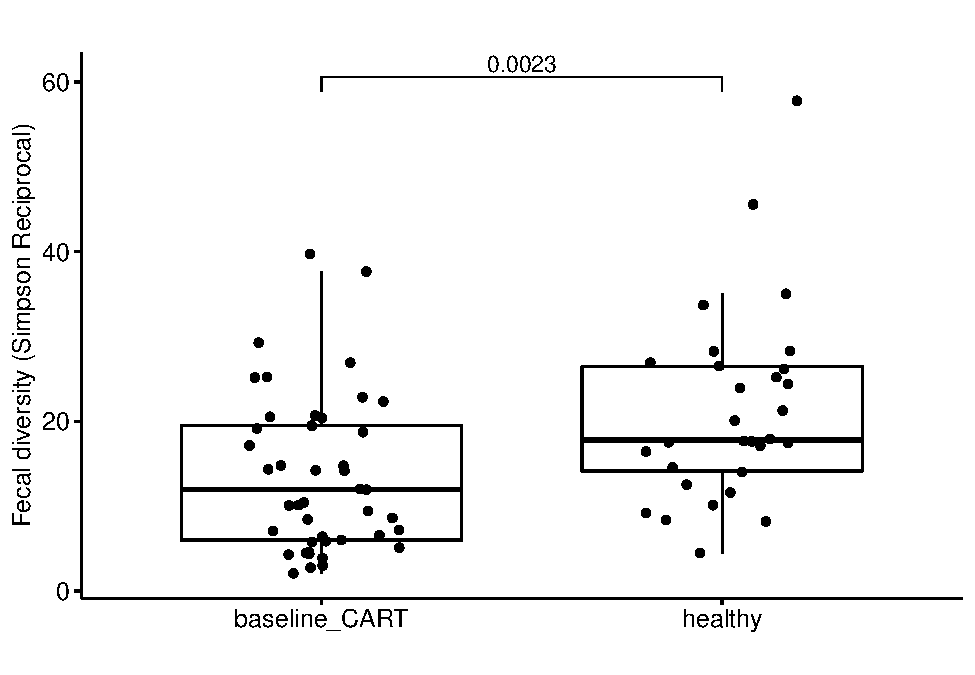
\includegraphics{analysis_files/figure-latex/unnamed-chunk-10-1.pdf}

\hypertarget{beta-diversity-pcoa-of-bray-curtis}{%
\subsection{beta diversity (PCOA of Bray-Curtis)}\label{beta-diversity-pcoa-of-bray-curtis}}

\begin{Shaded}
\begin{Highlighting}[]
\FunctionTok{library}\NormalTok{(vdbR)}
\FunctionTok{connect\_database}\NormalTok{(}\StringTok{\textquotesingle{}\textasciitilde{}/dbConfig.txt\textquotesingle{}}\NormalTok{)}

\NormalTok{healthy }\OtherTok{\textless{}{-}}\NormalTok{ healthy\_volunteers\_ag }\SpecialCharTok{\%\textgreater{}\%} 
  \FunctionTok{inner\_join}\NormalTok{(asv\_alpha\_diversity\_ag, }\AttributeTok{by =} \FunctionTok{c}\NormalTok{(}\StringTok{"sampleid"}\NormalTok{, }\StringTok{"oligos\_id"}\NormalTok{)) }
\NormalTok{cts }\OtherTok{\textless{}{-}} \FunctionTok{get\_counts\_subset}\NormalTok{(}\FunctionTok{c}\NormalTok{(stb}\SpecialCharTok{$}\NormalTok{sampleid, healthy }\SpecialCharTok{\%\textgreater{}\%} \FunctionTok{pull}\NormalTok{(sampleid)))}

\CommentTok{\# a total of 75 samples counts. there are 3 healthy samples I don\textquotesingle{}t have count .}
\NormalTok{nsamp }\OtherTok{\textless{}{-}}\NormalTok{ cts }\SpecialCharTok{\%\textgreater{}\%} 
  \FunctionTok{distinct}\NormalTok{(sampleid) }\SpecialCharTok{\%\textgreater{}\%} 
\NormalTok{  nrow}

\NormalTok{all\_pheno }\OtherTok{\textless{}{-}} \FunctionTok{bind\_rows}\NormalTok{(healthy }\SpecialCharTok{\%\textgreater{}\%} 
  \FunctionTok{select}\NormalTok{(sampleid) }\SpecialCharTok{\%\textgreater{}\%} 
  \FunctionTok{mutate}\NormalTok{(}\AttributeTok{grp =} \StringTok{\textquotesingle{}healthy\textquotesingle{}}\NormalTok{, }\AttributeTok{center =} \StringTok{\textquotesingle{}healthy\textquotesingle{}}\NormalTok{),}
\NormalTok{  stb }\SpecialCharTok{\%\textgreater{}\%} \FunctionTok{select}\NormalTok{(sampleid, center)  }\SpecialCharTok{\%\textgreater{}\%} 
    \FunctionTok{mutate}\NormalTok{(}\AttributeTok{grp =} \StringTok{\textquotesingle{}CART\textquotesingle{}}\NormalTok{) }\SpecialCharTok{\%\textgreater{}\%} 
    \FunctionTok{select}\NormalTok{(sampleid, grp, center)}
\NormalTok{  ) }\SpecialCharTok{\%\textgreater{}\%} 
\NormalTok{  ungroup }\SpecialCharTok{\%\textgreater{}\%} 
  \FunctionTok{distinct}\NormalTok{(sampleid, }\AttributeTok{.keep\_all =}\NormalTok{ T) }\SpecialCharTok{\%\textgreater{}\%} 
  \FunctionTok{inner\_join}\NormalTok{(asv\_alpha\_diversity\_ag }\SpecialCharTok{\%\textgreater{}\%} 
               \FunctionTok{distinct}\NormalTok{(sampleid, }\AttributeTok{.keep\_all =}\NormalTok{ T) }\SpecialCharTok{\%\textgreater{}\%} 
               \FunctionTok{distinct}\NormalTok{(path\_pool, sampleid))}


\CommentTok{\# filter \textgreater{}0.01\% in more than 25\% samples}
\NormalTok{keepa }\OtherTok{\textless{}{-}}\NormalTok{ cts }\SpecialCharTok{\%\textgreater{}\%} 
  \FunctionTok{filter}\NormalTok{(count\_relative }\SpecialCharTok{\textgreater{}} \FloatTok{0.0001}\NormalTok{) }\SpecialCharTok{\%\textgreater{}\%} 
  \FunctionTok{count}\NormalTok{(asv\_key) }\SpecialCharTok{\%\textgreater{}\%} 
  \FunctionTok{filter}\NormalTok{(n }\SpecialCharTok{\textgreater{}} \FunctionTok{floor}\NormalTok{(nsamp }\SpecialCharTok{*} \FloatTok{0.25}\NormalTok{)) }\SpecialCharTok{\%\textgreater{}\%} 
  \FunctionTok{pull}\NormalTok{(asv\_key)}

\NormalTok{cts\_fil }\OtherTok{\textless{}{-}}\NormalTok{ cts }\SpecialCharTok{\%\textgreater{}\%} 
  \FunctionTok{filter}\NormalTok{(asv\_key }\SpecialCharTok{\%in\%}\NormalTok{ keepa) }\SpecialCharTok{\%\textgreater{}\%} 
  \FunctionTok{select}\NormalTok{(sampleid, asv\_key,count\_relative ) }\SpecialCharTok{\%\textgreater{}\%} 
  \FunctionTok{spread}\NormalTok{(}\AttributeTok{key =} \StringTok{\textquotesingle{}asv\_key\textquotesingle{}}\NormalTok{, }\AttributeTok{value =} \StringTok{\textquotesingle{}count\_relative\textquotesingle{}}\NormalTok{, }\AttributeTok{fill =} \DecValTok{0}\NormalTok{) }\SpecialCharTok{\%\textgreater{}\%} 
  \FunctionTok{column\_to\_rownames}\NormalTok{(}\StringTok{\textquotesingle{}sampleid\textquotesingle{}}\NormalTok{)}

\FunctionTok{library}\NormalTok{(vegan)}
\NormalTok{dist\_ }\OtherTok{\textless{}{-}} \FunctionTok{vegdist}\NormalTok{(cts\_fil, }\AttributeTok{method =} \StringTok{\textquotesingle{}bray\textquotesingle{}}\NormalTok{)}
\NormalTok{eigen }\OtherTok{\textless{}{-}} \FunctionTok{pcoa}\NormalTok{(dist\_)}\SpecialCharTok{$}\NormalTok{values}\SpecialCharTok{$}\NormalTok{Eigenvalues}
\NormalTok{percent\_var }\OtherTok{\textless{}{-}} \FunctionTok{signif}\NormalTok{(eigen}\SpecialCharTok{/}\FunctionTok{sum}\NormalTok{(eigen), }\DecValTok{3}\NormalTok{)}\SpecialCharTok{*}\DecValTok{100}

\NormalTok{bc }\OtherTok{\textless{}{-}} \FunctionTok{cmdscale}\NormalTok{(dist\_, }\AttributeTok{k =} \DecValTok{2}\NormalTok{)}

\NormalTok{bc }\SpecialCharTok{\%\textgreater{}\%}
  \FunctionTok{as.data.frame}\NormalTok{() }\SpecialCharTok{\%\textgreater{}\%}
  \FunctionTok{rownames\_to\_column}\NormalTok{(}\StringTok{\textquotesingle{}sampleid\textquotesingle{}}\NormalTok{) }\SpecialCharTok{\%\textgreater{}\%} 
  \FunctionTok{ungroup}\NormalTok{() }\SpecialCharTok{\%\textgreater{}\%} 
  \FunctionTok{inner\_join}\NormalTok{(all\_pheno) }\SpecialCharTok{\%\textgreater{}\%} 
  \FunctionTok{distinct}\NormalTok{() }\SpecialCharTok{\%\textgreater{}\%} 
  \FunctionTok{ggscatter}\NormalTok{(}\AttributeTok{x =} \StringTok{\textquotesingle{}V1\textquotesingle{}}\NormalTok{, }\AttributeTok{y =} \StringTok{\textquotesingle{}V2\textquotesingle{}}\NormalTok{, }\AttributeTok{color =}  \StringTok{\textquotesingle{}grp\textquotesingle{}}\NormalTok{) }\SpecialCharTok{+}
  \FunctionTok{labs}\NormalTok{(}\AttributeTok{title =} \StringTok{\textquotesingle{}PCOA of healthy and CART patients\textquotesingle{}}\NormalTok{) }\SpecialCharTok{+}
  \FunctionTok{xlab}\NormalTok{(}\FunctionTok{paste0}\NormalTok{(}\StringTok{"PC 1 ["}\NormalTok{,percent\_var[}\DecValTok{1}\NormalTok{],}\StringTok{"\%]"}\NormalTok{)) }\SpecialCharTok{+}
  \FunctionTok{ylab}\NormalTok{(}\FunctionTok{paste0}\NormalTok{(}\StringTok{"PC 2 ["}\NormalTok{,percent\_var[}\DecValTok{2}\NormalTok{],}\StringTok{"\%]"}\NormalTok{)) }\SpecialCharTok{+}
  \CommentTok{\#theme\_void() +}
  \FunctionTok{ggsave}\NormalTok{(}\StringTok{\textquotesingle{}figs/PCOA(bray{-}curtis) of healthy and CART patients.pdf\textquotesingle{}}\NormalTok{)}
\end{Highlighting}
\end{Shaded}

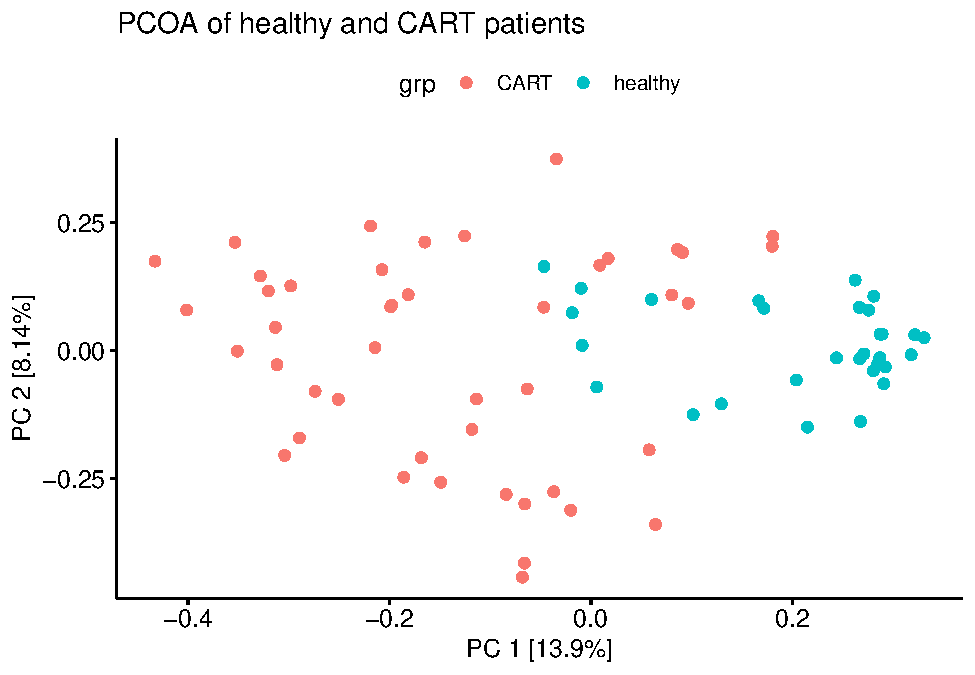
\includegraphics{analysis_files/figure-latex/unnamed-chunk-11-1.pdf}

\begin{Shaded}
\begin{Highlighting}[]
\CommentTok{\# a pcoa at asv level to show they are from different pools and well mixed }
\NormalTok{cts }\OtherTok{\textless{}{-}} \FunctionTok{get\_counts\_subset}\NormalTok{(}\FunctionTok{c}\NormalTok{(stb}\SpecialCharTok{$}\NormalTok{sampleid))}

\CommentTok{\# filter \textgreater{}0.01\% in more than 25\% samples}
\NormalTok{keepa }\OtherTok{\textless{}{-}}\NormalTok{ cts }\SpecialCharTok{\%\textgreater{}\%} 
  \FunctionTok{filter}\NormalTok{(count\_relative }\SpecialCharTok{\textgreater{}} \FloatTok{0.0001}\NormalTok{) }\SpecialCharTok{\%\textgreater{}\%} 
  \FunctionTok{count}\NormalTok{(asv\_key) }\SpecialCharTok{\%\textgreater{}\%} 
  \FunctionTok{filter}\NormalTok{(n }\SpecialCharTok{\textgreater{}} \FunctionTok{floor}\NormalTok{(nsamp }\SpecialCharTok{*} \FloatTok{0.25}\NormalTok{)) }\SpecialCharTok{\%\textgreater{}\%} 
  \FunctionTok{pull}\NormalTok{(asv\_key)}

\NormalTok{cts\_fil }\OtherTok{\textless{}{-}}\NormalTok{ cts }\SpecialCharTok{\%\textgreater{}\%} 
  \FunctionTok{filter}\NormalTok{(asv\_key }\SpecialCharTok{\%in\%}\NormalTok{ keepa) }\SpecialCharTok{\%\textgreater{}\%} 
  \FunctionTok{select}\NormalTok{(sampleid, asv\_key,count\_relative ) }\SpecialCharTok{\%\textgreater{}\%} 
  \FunctionTok{spread}\NormalTok{(}\AttributeTok{key =} \StringTok{\textquotesingle{}asv\_key\textquotesingle{}}\NormalTok{, }\AttributeTok{value =} \StringTok{\textquotesingle{}count\_relative\textquotesingle{}}\NormalTok{, }\AttributeTok{fill =} \DecValTok{0}\NormalTok{) }\SpecialCharTok{\%\textgreater{}\%} 
  \FunctionTok{column\_to\_rownames}\NormalTok{(}\StringTok{\textquotesingle{}sampleid\textquotesingle{}}\NormalTok{)}

\NormalTok{dist\_ }\OtherTok{\textless{}{-}} \FunctionTok{vegdist}\NormalTok{(cts\_fil, }\AttributeTok{method =} \StringTok{\textquotesingle{}bray\textquotesingle{}}\NormalTok{)}
\NormalTok{eigen }\OtherTok{\textless{}{-}} \FunctionTok{pcoa}\NormalTok{(dist\_)}\SpecialCharTok{$}\NormalTok{values}\SpecialCharTok{$}\NormalTok{Eigenvalues}
\NormalTok{percent\_var }\OtherTok{\textless{}{-}} \FunctionTok{signif}\NormalTok{(eigen}\SpecialCharTok{/}\FunctionTok{sum}\NormalTok{(eigen), }\DecValTok{3}\NormalTok{)}\SpecialCharTok{*}\DecValTok{100}

\NormalTok{bc }\OtherTok{\textless{}{-}} \FunctionTok{cmdscale}\NormalTok{(dist\_, }\AttributeTok{k =} \DecValTok{2}\NormalTok{)}

\NormalTok{mp }\OtherTok{\textless{}{-}}\NormalTok{ bc }\SpecialCharTok{\%\textgreater{}\%}
  \FunctionTok{as.data.frame}\NormalTok{() }\SpecialCharTok{\%\textgreater{}\%}
  \FunctionTok{rownames\_to\_column}\NormalTok{(}\StringTok{\textquotesingle{}sampleid\textquotesingle{}}\NormalTok{) }\SpecialCharTok{\%\textgreater{}\%} 
  \FunctionTok{ungroup}\NormalTok{() }\SpecialCharTok{\%\textgreater{}\%} 
  \FunctionTok{inner\_join}\NormalTok{(all\_pheno) }\SpecialCharTok{\%\textgreater{}\%} 
  \FunctionTok{distinct}\NormalTok{(sampleid, }\AttributeTok{.keep\_all =}\NormalTok{ T)  }\SpecialCharTok{\%\textgreater{}\%} 
  \FunctionTok{mutate}\NormalTok{(}\AttributeTok{pool =} \FunctionTok{str\_extract}\NormalTok{(path\_pool, }\StringTok{\textquotesingle{}Sample.+/\textquotesingle{}}\NormalTok{)) }\SpecialCharTok{\%\textgreater{}\%} 
  \FunctionTok{mutate}\NormalTok{(}\AttributeTok{pool =} \FunctionTok{str\_replace}\NormalTok{(pool, }\StringTok{\textquotesingle{}Sample\_\textquotesingle{}}\NormalTok{,}\StringTok{\textquotesingle{}\textquotesingle{}}\NormalTok{)) }\SpecialCharTok{\%\textgreater{}\%} 
  \FunctionTok{mutate}\NormalTok{(}\AttributeTok{pool =} \FunctionTok{if\_else}\NormalTok{(}\FunctionTok{str\_detect}\NormalTok{(pool, }\StringTok{\textquotesingle{}IGO\textquotesingle{}}\NormalTok{), }\FunctionTok{str\_extract}\NormalTok{(pool, }\StringTok{\textquotesingle{}IGO.+$\textquotesingle{}}\NormalTok{), pool)) }\SpecialCharTok{\%\textgreater{}\%} 
  \FunctionTok{mutate}\NormalTok{(}\AttributeTok{pool =} \FunctionTok{str\_replace}\NormalTok{(pool, }\StringTok{\textquotesingle{}\_1/|\_comple.+$\textquotesingle{}}\NormalTok{,}\StringTok{\textquotesingle{}\textquotesingle{}}\NormalTok{))}

\NormalTok{mp }\SpecialCharTok{\%\textgreater{}\%} 
  \FunctionTok{ggscatter}\NormalTok{(}\AttributeTok{x =} \StringTok{\textquotesingle{}V1\textquotesingle{}}\NormalTok{, }\AttributeTok{y =} \StringTok{\textquotesingle{}V2\textquotesingle{}}\NormalTok{, }\AttributeTok{color =}  \StringTok{\textquotesingle{}pool\textquotesingle{}}\NormalTok{, }\AttributeTok{size =} \DecValTok{3}\NormalTok{) }\SpecialCharTok{+}
  \FunctionTok{labs}\NormalTok{(}\AttributeTok{title =} \StringTok{\textquotesingle{}PCOA of CART patients\textquotesingle{}}\NormalTok{) }\SpecialCharTok{+}
  \FunctionTok{xlab}\NormalTok{(}\FunctionTok{paste0}\NormalTok{(}\StringTok{"PC 1 ["}\NormalTok{,percent\_var[}\DecValTok{1}\NormalTok{],}\StringTok{"\%]"}\NormalTok{)) }\SpecialCharTok{+}
  \FunctionTok{ylab}\NormalTok{(}\FunctionTok{paste0}\NormalTok{(}\StringTok{"PC 2 ["}\NormalTok{,percent\_var[}\DecValTok{2}\NormalTok{],}\StringTok{"\%]"}\NormalTok{)) }\SpecialCharTok{+}
  \CommentTok{\#theme\_void() +}
  \FunctionTok{ggsave}\NormalTok{(}\StringTok{\textquotesingle{}figs/PCOA(bray{-}curtis) (ASV level)of CART patients\_pool.pdf\textquotesingle{}}\NormalTok{, }\AttributeTok{width =} \DecValTok{9}\NormalTok{, }\AttributeTok{height =} \DecValTok{9}\NormalTok{)}
\end{Highlighting}
\end{Shaded}

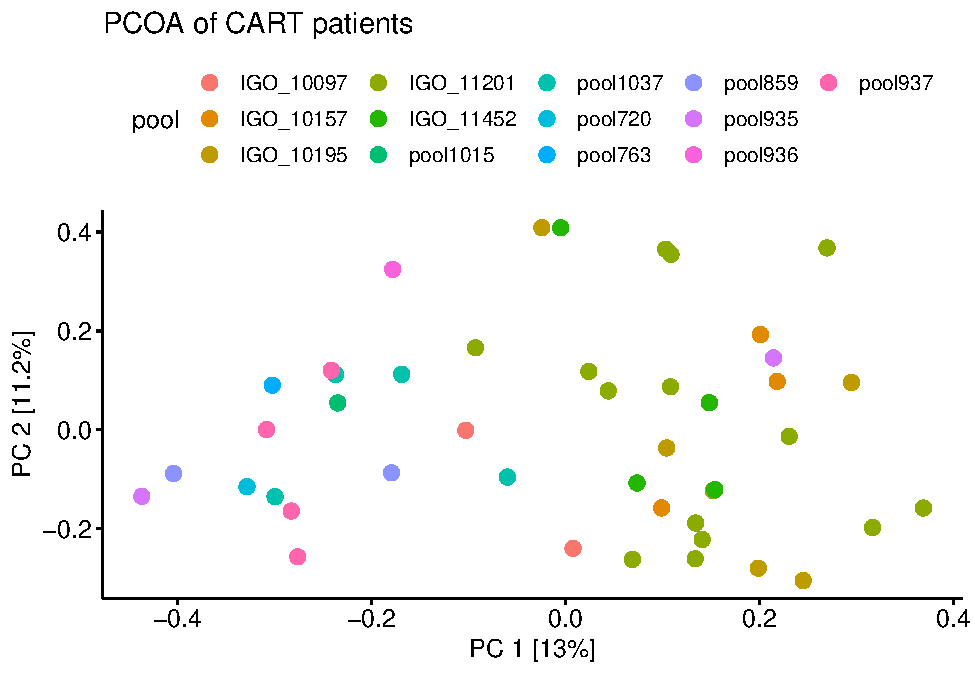
\includegraphics{analysis_files/figure-latex/unnamed-chunk-12-1.pdf}

\hypertarget{methods}{%
\chapter{Methods}\label{methods}}

We describe our methods in this chapter.
aklalallla

\hypertarget{applications}{%
\chapter{Applications}\label{applications}}

Some \emph{significant} applications are demonstrated in this chapter.

\hypertarget{example-one}{%
\section{Example one}\label{example-one}}

\hypertarget{example-two}{%
\section{Example two}\label{example-two}}

\hypertarget{final-words}{%
\chapter{Final Words}\label{final-words}}

We have finished a nice book.

  \bibliography{book.bib,packages.bib}

\end{document}
